\documentclass[a4paper,10pt,fleqn,oneside]{scrartcl}
\usepackage[usenames,dvipsnames]{xcolor}
\usepackage[english]{babel}
\usepackage[utf8]{inputenc}
\usepackage[T1]{fontenc}
\usepackage[toc,page]{appendix}
\usepackage{floatflt}
\usepackage{lmodern}
\usepackage{amssymb}
\usepackage{amsmath}
\usepackage{enumerate}
\usepackage{enumitem}
\usepackage{fancyhdr}
\usepackage{pgfplots}
\usepackage{multicol}
\usepackage{tikz}
\usepackage[hidelinks]{hyperref}
\usepackage{listings}
\usepackage{mdframed}
\usepackage{tabularx}
\usepackage{tabu}
\usepackage{multirow}
\usepackage{booktabs}
\usepackage{pgfplots}
\usepackage{pgfplotstable}
\usepackage{float}
\usepackage{wrapfig}
\usepackage{blindtext}
\usepackage{etoolbox}
\usepackage{lastpage}
\usepackage{tocloft}
\usepackage{graphicx}
\usepackage{caption}
\usepackage{subcaption}
\usepackage[asymmetric,top=1.5in,bottom=1.5in,left=1.2in,right=1.2in]{geometry}
\usepackage[sectionbib]{natbib}
\interfootnotelinepenalty=10000

\usepackage{tgpagella}
% \usepackage{quattrocento}

\usetikzlibrary{shapes,arrows,calc,patterns,decorations.markings,shadows.blur}


\title{A prototype for a typing device using IMUs and machine learning}
\subtitle{Exposé for two Bachelor of Science theses}
\author{
  Bienkowski, Paul\\
  \texttt{2bienkow@informatik.uni-hamburg.de}
  \and
  Konietzny, Carolin\\
  \texttt{3konietz@informatik.uni-hamburg.de}
}
\date{\today}

\pagestyle{fancy}
\fancyhf{}
\fancyhead[L]{Exposé - Typing device}
% \fancyhead[R]{}
%\setlength{\footskip}{2em}
%\setlength{\footrulewidth}{0.4pt}
\fancyfoot[L]{\small{}Bienkowski, Konietzny}
\fancyfoot[R]{\small{}Page \thepage \:of \pageref{LastPage}}

\newif\iffinal
\finaltrue

% \renewcommand{\arraystretch}{1.2}
% \renewcommand{\arraystretch}{1.5}
% \renewcommand{\familydefault}{\sfdefault}
\linespread{1.1}

\let\stdsection\section
% \renewcommand\section{\newpage\stdsection}
\setlength{\parindent}{0pt}
% \setlength{\parskip}{1.8ex}
\setlength{\parskip}{1.0ex}

\begin{document}

\maketitle
\tableofcontents

\section{Introduction}
\subsection{Motivation}
The 21\textsuperscript{st} century is a time where one technology chases the other, everything new is the older version of tomorrow. Smartphones getting faster, smartwatches support the use of the phone. Virtual reality fascinates more and more people, even the TV is almost on a par with real persons in relation to communication and interaction.
One limiting thing of getting even smaller devices is the need of a possibility to interact with the device, such as keyboards or mouse cursors. Even with voice recognition getting better and better, keyboards are still an important tool to interact. Wether it is for fast programming or to write texts, the comfort of typing fast and an great amount of characters is very important.
One of the main reasons for our prototype is the fact that every keyboards needs its space. Even the small ones are often the limiting size of a device.  
The position of the keys is fixed in most of the cases. The user can remap the characters, but not the position of the key itself. Therefore the user can't personalize the keyboard which is bad in many cases.
For example persons who can't write the recommendet touch system (maybe because of deficient exercise or because of a lack of fingers).
There are many disadvantages of a keyboard, bot nonetheless typing is very effective and precise.
The goal is to make typing even more comfortable. Getting rid of the hardware and increasing the ergonomy of typing itself. Without the hardware and with own finger movements, typing will become an effective and fitting way to interact with machines.


% * tastaturen sind doof
%   - unhandlich
%   - geräte werden kleiner, aber nicht unbegrenzt wegen tastaturen
%   - sehnenscheidenentzündungen, erkrankung der unterarmmuskulatur (mikro risse) etc
%   - man muss immer an einem tisch sitzen, tippen im stehen ist einfach doof
%   - schwer anpassbar an körperliche fähigkeiten (vorgegebene, fixe anordnung)
%     * 10-Finger-tippen ist gar nicht so toll für Jedermann (Fingermangel, ...)
% * tippen ist cool
%   - wichtig ist präzise Eingabe von hunderten von zeichen (programmieren!)
%   - soll schnell sein
% * wir wollen tippen (zeicheneingabe) ohne tastatur, 
%   - flexibel
%   - keine große hardware


\subsection{Goal}

We want to create a new device that maps hand and finger movements to key
presses -- just like a traditional keyboard, but without the bulky and
restraining hardware that's currently required for keyboard input.

To do so, we want to attach multiple movement sensors (inertial measurement
units, IMUs\footnote{These usually combine multidimensional gyroscopes,
accelerometers and magnetometers in one package, giving us access to the linear
and angular acceleration as well as absolute orientation of the device.}) to
different parts of the hand and record their outputs, including the
corresponding keystrokes from an actual keyboard.

We will then analyze the collected data to learn how hand movements translate
into keystrokes. To do so, we will use a machine learning algorithm that can
later be fed with live sensor data to replace the tranditional keyboard in
generating the keystrokes.

We believe a neural network is very suitable for this task, as it might be able
to detect small differences in the way the user pushes different keys that are
not predicable and specific for the actual user. Our goal is therefore not to
create a universally applicable device, but learn one person's typing gestures
with adequate accuracy to be usable as an input device.

\subsection{Vision}

If our experimental prototype proves to be suitable for precise keyboard input,
we can envision to take the idea further.

\begin{itemize}
    \item Make the device universally applicable, without the need to
    train a complex network. Collect more data to generalize better and provide
    a ``starting point'' for customized user profiles.
    \item Optimize the hardware. Make it lighter, smaller, more robust,
    cheaper.  Replace wires with wireless connections. 
    \item Use sensor data from hardware for robotics applications.
    \item Use the same hardware and principle to replace other input
    devices, e.g. piano keyboard, braille typing device, gesture recognition.
    \item Improve ergonomic properties.
    \item Perform online learning\footnote{keep learning from the system's own
    output to keep track of small adjustments over time} to move away from the
    predetermined key layout of traditional keyboards.  
\end{itemize}

\section{Project}

\subsection{Overview}

In figure~\ref{fig:overview} we identify the planned architecture of our product, including
its physical and software parts and their interaction with each other.

\begin{figure}
    \centering
    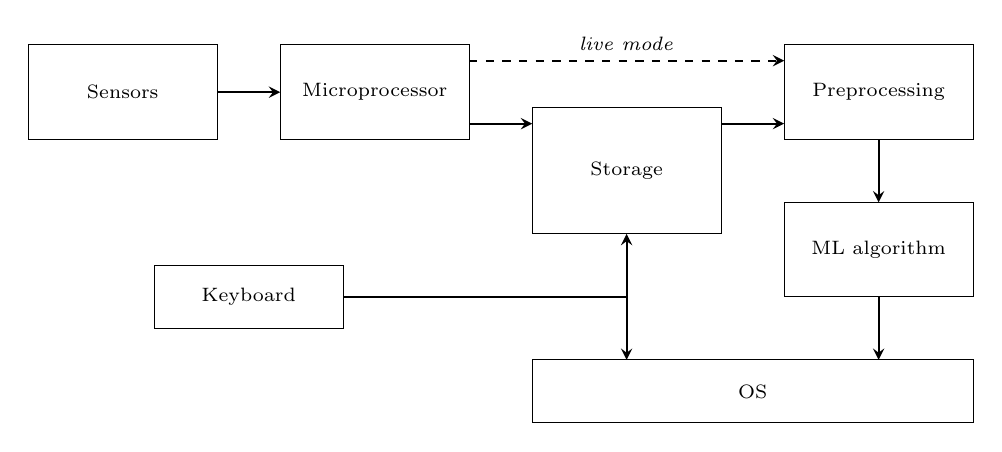
\begin{tikzpicture}[every node/.style={font=\scriptsize},scale=0.8]
        \tikzstyle{arrow} = [thick,->,>=stealth]
        \draw (0,0) rectangle (3,1.5) node[pos=.5] {Sensors};
        \draw (4,0) rectangle (7,1.5) node[pos=.5] {Microprocessor};
        \draw (2,-2) rectangle (5,-3) node[pos=.5] {Keyboard};
        \draw (8,0.5) rectangle (11,-1.5) node[pos=.5] {Storage};
        \draw (12,0) rectangle (15,1.5) node[pos=.5] {Preprocessing};
        \draw (12,-1) rectangle (15,-2.5) node[pos=.5] {ML algorithm};
        \draw (8,-3.5) rectangle (15,-4.5) node[pos=.5] {OS};

        \draw [arrow] (3, 0.75) -- (4, 0.75);
        \draw [arrow] (7, 0.25) -- (8, 0.25);
        \draw [arrow] (11, 0.25) -- (12, 0.25);
        \draw [arrow] (13.5, 0) -- (13.5, -1);
        \draw [arrow] (13.5, -2.5) -- (13.5, -3.5);
        \draw [arrow] (5, -2.5) -| (9.5, -1.5);
        \draw [arrow] (5, -2.5) -| (9.5, -3.5);
        \draw [dashed, arrow] (7, 1.25) -- node[anchor=south]{\textit{live mode}}(12, 1.25);
    \end{tikzpicture}
    \caption{Project overview}
    \label{fig:overview}
\end{figure}


For planning, building and connecting the hardware device, we will seek
assistance from the group Technical Aspects of Multimodal Systems (TAMS) from the
Department of Informatics of the University of Hamburg.

For developing the major software parts (preprocessing and machine learning) we
are looking forward to a  cooperation with the group Knowledge Technology
(WTM), also from the Department of Informatics of the University of Hamburg.

\subsection{Scope}

We shall now express the foreseeable scope of the project:

For the hardware device we first have to research suitable components and order
these. We have listed an estimation of the required hardware components including
their prices in Table~\ref{tbl:pricesheet}.

\begin{table}[htb]
    \centering
    \begin{tabu}{lrrr}
        \tabucline[1pt]{-} 
        \textbf{Component} & \textbf{EUR/unit} & \textbf{Count} & \textbf{Total/EUR} \\
        \tabucline[1pt]{-} 
        IMU & 10-20 & 12 & 120-240 \\
        Processor & 20-50 & 1-2 & 40-100 \\
        Other & TBD & TBD & 0-100 \\
        \tabucline[1pt]{-} 
        \textbf{Total} &  &  & 160-340 \\
        \tabucline[1pt]{-} 
    \end{tabu}
    \caption{Estimated hardware requirements and costs}
    \label{tbl:pricesheet}
\end{table}

For the hardware part we will also have to work out how to actually connect the
sensors to the processor(s), retrieve data from the sensors, and transmit them
to the computer. We will also have to actually build the device and find a way
to attach the hardware to the hand without impeding hand movements too much.

For the software part, we will have to build some scaffolding to pass around
data between our different software components and into the operating system.
We need to write the recording software for generating learning and testing
datasets, and the preprocessing code. We will probably find some configurable
implementation of a suitable machine learning algorithm (which we have to
choose first), so we do not plan to implement that part ourselves.

We expect that the hardest problem to solve will be defining and implementing
the preprocessing steps as well as choosing and configuring the machine
learning algorithm.

Our main intent is to define suitable preprocessing methods for the task at
hand.  We do not expect to get fancy with the machine learning part initially,
instead we aim to use something simple and fast for the proof of concept. We
are considering neural networks, specifically simple recurrent networks, to be
suitable for this task. However, evaluation of this assumption shall be part of
our works.

Of course all our attempts need to be evaluated, so we also have to define
performance metrics and evaluate our system against these. Since we're able to
learn offline with recorded data, it will be possible to repeat experiments
with different parameters to find good configurations.

In figure~\ref{fig:toc} we outline our preliminary table of contents. 


\begin{figure}[htb]
    \centering
    \begin{minipage}{0.8\textwidth}
        \renewcommand{\labelenumii}{\theenumii}
        \renewcommand{\theenumii}{\theenumi.\arabic{enumii}.}

        \begin{enumerate}[noitemsep]
            \item Introduction
                \begin{enumerate}[noitemsep]
                    \item Idea
                    \item Vision
                    \item Project scope
                \end{enumerate}

            \item State of the art

            \item Initial hardware development
                \begin{enumerate}[noitemsep]
                    \item Component research
                    \item Connection
                    \item Data transmission and retrieval
                    \item Ergonomic improvements
                \end{enumerate}

            \item Initial software development
                \begin{enumerate}[noitemsep]
                    \item Preprocessing
                    \item Machine learning
                \end{enumerate}

            \item Evaluation 
                \begin{enumerate}[noitemsep]
                    \item Methods
                    \item Results
                \end{enumerate}

            \item Improvements
            \item Discussion
            \item Outlook
            \item References
        \end{enumerate}
    \end{minipage}
    \caption{Preliminary table of contents}
    \label{fig:toc}
\end{figure}

\section{State of the Art}
Detection of finger and hand movements is a very complex and widespread subject. There is lots of research being done to match the movement of the fingers to different actions and commands for a machine.

One device using IMUs is the \textsc{InerTouchHand}, developed in Portugal. It is capable to track finger movements by using eleven IMUs on each hand. They use relative positioning of the fingers to the back of the hands to match the finger and hand positions to predefined gestures of the Portuguese Sign Language \cite{inertouchhand}. One big difference to the product we are planning are the predefined gestures which the system is able to match to. Our approach is to learn the gestures by using tagged data. Doing so we might be able to learn gestures without knowing the exact movements beforehand.

Another project is \textsc{cavallo-senshand-parkinsons}, which uses 4 IMUs, each of them with 9 degrees of freedom. In \cite{cavallo-senshand-parkinsons} they use SensHand to examine movements of people with Parkinson's disease.

There are many more projects which use hand movements to interact with machines. Some using camrea tracking systems \cite{ellithorpe-kinect-typing}, flex sensors or EMGs \cite{imu-emg}.

Our approach is to link the hardware side and the software side by using IMUs and a learning algorithm to not only learn movements the human eye can detect (like moving the little finger towards the delete button) but also learn about other movements (such as lifting the middlefinger while the little finger reaches for the delete button). With this approach we are hoping to find a way to get rid of the need for a constricting keyboard.

We couldn't find another project that combines the use of IMUs and machine learning to replace a keyboard.
Some projects use machine learning \cite{ellithorpe-kinect-typing}, using cameras instead of IMUs. Others are simulating a keyboard without the use of machine learning, using a top-down approach to map movements to predefined movements for specific characters.


% \newpage

\nocite{*}
\bibliographystyle{plain}
\bibliography{bibliography}
% \listoffigures
% \listoftables



\end{document}
